% Author Name: Enrique Pérez
% Author Contact: enrique.perez2@um.es
% Version: 1.0.1 - 2025/05/17
% Public Repository: https://github.com/enriiquee/umu-thesis

% En el repositorio público puedes encontrar las instrucciones más detalladas. 

%%% Document Options %%%
\documentclass[
    language=english,
    docstage=final,
    media=paper,
    linkcolor=black!45!black,
    chapterstyle=fancy,
]{UMUthesis} % Refer to the Wiki for a list of available options.

%%% Document Version %%%
\DocumentVersion{1.0.0} % This is required only if the 'docstage' is set to 'working'.

%%% Document Metadata %%%
% First Author (Mandatory)
\FirstAuthor{Andrés Maglione}

% Supervisor (Mandatory)
\Supervisor{Dra. Ana Carolina Olivera}
\SupervisorMail{Johnwick@gmail.com}

% Title (Mandatory) if it's international 
\Title{English title of the thesis }

% Title spanish (Mandatory)
\TitleEsp{Título en español de la tesis}

% University (Mandatory)
\University{Universidad Nacional de Cuyo}

% Local & Date (Mandatory)
\Date{Murcia, \DTMmonthname{\month} \number\year}



%%% Loading of Glossary and Acronyms %%%
\makeglossaries
\loadglsentries{Matter/04-Glossary}
\loadglsentries[\acronymtype]{Matter/05-Acronyms}

\begin{document}

%%% Front Matter %%%
% ----------------------------------------
% Definición del fondo 
% ----------------------------------------
  \newcommand\BackgroundPicCover{%
    \put(0,0){%
      \parbox[b][\paperheight]{\paperwidth}{%
        \vfill
        \centering
        
\includegraphics[width=\paperwidth,height=\paperheight,keepaspectratio]{Figures/Theme/Front-Page.pdf}%
        \vfill
      }%
    }%
  } %

\AddToShipoutPictureBG*{\BackgroundPicCover}

% ----------------------------------------
% Portada con cambio según LanguageOption
% ----------------------------------------
\newgeometry{
  top=1.5cm, bottom=1.77cm,
  left=2cm, right=1.5cm,
  bindingoffset=0cm
}
\begin{titlepage}
  \AddToShipoutPictureBG*{\BackgroundPicCover}
  \begingroup
    \plexsans %  Aplica IBM Plex Sans solo localmente

    % Color de texto según opción de portada
    \color{white}
    
    \vspace*{\fill}  % empuje vertical

    % Selección de portada en inglés vs español
    \ifthenelse{\equal{\LanguageOption}{english}}{%
      % ======= PORTADA EN INGLÉS =======
      {\noindent\bfseries\fontsize{12}{14}\selectfont TESINA FINAL DE CARRERA\par}
      \vspace{0.5cm}
      {\noindent\raggedright\itshape\fontsize{22}{24}\selectfont \titleesp\par}
      \vspace{2cm}

      \noindent
      \begin{minipage}[t]{0.40\textwidth}
        \raggedright
        {\itshape\fontsize{14}{20}\selectfont \thetitle\par}
      \end{minipage}%
      \begin{minipage}[t]{0.4\textwidth}
        \raggedright
        \begin{tabbing}
          \hspace{4cm}\=\kill
          \textbf{\fontsize{12}{10}\selectfont AUTHOR:}\> \GetFirstAuthor \\[0.3cm]
          \textbf{\fontsize{12}{10}\selectfont SUPERVISORS:}\> \GetSupervisor   \\
                                            
        \end{tabbing}
      \end{minipage}%
      \begin{minipage}[t]{0.1\textwidth}
        \vspace{1.5cm}
        \raggedleft
        {\fontsize{13}{16}\selectfont \the\year \par}
      \end{minipage}
    }{%
      % ======= PORTADA EN ESPAÑOL =======
      {\noindent\bfseries\fontsize{12}{14}\selectfont TESINA FINAL DE CARRERA\par}
      \vspace{0.5cm}
      {\noindent\raggedright\itshape\fontsize{22}{24}\selectfont \titleesp\par}
      \vspace{2cm}

      \noindent
      
      \begin{minipage}[t]{0.4\textwidth}
        \raggedright
        \begin{tabbing}
          \hspace{4cm}\=\kill
          \textbf{\fontsize{12}{10}\selectfont AUTOR:}\> \GetFirstAuthor \\[0.3cm]
          \textbf{\fontsize{12}{10}\selectfont DIRECTORA:}\> \GetSupervisor   \\

        \end{tabbing}
      \end{minipage}%
      \begin{minipage}[t]{0.45\textwidth}
        \vspace{2cm}
        \raggedleft
        {\fontsize{13}{16}\selectfont \the\year \par}
      \end{minipage}
    }
    % Fin condicional LanguageOption

    \vspace{1cm}
  \endgroup
\end{titlepage}
\restoregeometry
\MediaOptionLogicBlank
% ----------------------------------------
% Definición del fondo 
% ----------------------------------------
  \newcommand\BackgroundPicCoverWhite{%
    \put(0,0){%
      \parbox[b][\paperheight]{\paperwidth}{%
        \vfill
        \centering
        
\includegraphics[width=\paperwidth,height=\paperheight,keepaspectratio]{Figures/Theme/BG_UMU_White.pdf}%
        \vfill
      }%
    }%
  }%


\AddToShipoutPictureBG*{\BackgroundPicCoverWhite}

% ----------------------------------------
% Portada con cambio según LanguageOption
% ----------------------------------------
\newgeometry{
  top=1.5cm, bottom=1.77cm,
  left=1.5cm, right=1.5cm,
  bindingoffset=0cm
}
\begin{titlepage}
  \AddToShipoutPictureBG*{\BackgroundPicCoverWhite}
  \begingroup
    \plexsans % Aplica IBM Plex Sans solo localmente
    % Color de texto según opción de portada
    \color{black}

\vspace*{\fill}  % empuje vertical

    % Selección de portada en inglés vs español
\ifthenelse{\equal{\LanguageOption}{english}}{%
      % ======= PORTADA EN INGLÉS =======
      {\noindent\bfseries\fontsize{12}{14}\selectfont DOCTORAL THESIS\par}
      \vspace{0.5cm}
      {\noindent\raggedright\itshape\fontsize{22}{24}\selectfont \titleesp\par}
      \vspace{2cm}

      \noindent
      \begin{minipage}[t]{0.40\textwidth}
        \raggedright
        {\itshape\fontsize{14}{20}\selectfont \thetitle\par}
      \end{minipage}%
      \begin{minipage}[t]{0.4\textwidth}
        \raggedright
        \begin{tabbing}
          \hspace{4cm}\=\kill
          \textbf{\fontsize{12}{10}\selectfont AUTHOR:}\> \GetFirstAuthor \\[0.3cm]
          \textbf{\fontsize{12}{10}\selectfont SUPERVISORS:}\> \GetSupervisor   \\
                                              \> \GetCoSupervisor    \\
                                              \> \GetSecCoSupervisor
        \end{tabbing}
      \end{minipage}%
      \begin{minipage}[t]{0.1\textwidth}
        \vspace{1.5cm}
        \raggedleft
        {\fontsize{13}{16}\selectfont \the\year \par}
      \end{minipage}
    }{%
      % ======= PORTADA EN ESPAÑOL =======
      {\noindent\bfseries\fontsize{12}{14}\selectfont TESIS DOCTORAL\par}
      \vspace{0.5cm}
      {\noindent\raggedright\itshape\fontsize{22}{24}\selectfont \titleesp\par}
      \vspace{2cm}

      \noindent
      
      \begin{minipage}[t]{0.4\textwidth}
        \raggedright
        \begin{tabbing}
          \hspace{4cm}\=\kill
          \textbf{\fontsize{12}{10}\selectfont AUTOR:}\> \GetFirstAuthor \\[0.3cm]
          \textbf{\fontsize{12}{10}\selectfont DIRECTORES:}\> \GetSupervisor   \\
                                              \> \GetCoSupervisor    \\
                                              \> \GetSecCoSupervisor
        \end{tabbing}
      \end{minipage}%
      \begin{minipage}[t]{0.45\textwidth}
        \vspace{2cm}
        \raggedleft
        {\fontsize{13}{16}\selectfont \the\year \par}
      \end{minipage}
    }
   % Fin condicional LanguageOption

    \vspace{1cm}
  \endgroup
\end{titlepage}
\restoregeometry
\MediaOptionLogicBlank

%%% Copyright Statement %%%
\pagenumbering{gobble} % Prevent page numbering.

\thispagestyle{plain} % Page style without header and footer

\MediaOptionLogic

%%% Roman Numeration %%%
\pagenumbering{roman}

%%% Dedication %%%
\pagenumbering{gobble} % Prevent page numbering.
\chapter*{} % Chapter* to appear without numeration


\begin{flushright}
    \textit{A quien le dedicas la tesis. \\~\\ A tus padres o al profesor ese que nunca confió en ti. }
\end{flushright}



%%% Frase celebre %%%
\chapter*{} % Chapter* to appear without numeration

\begin{flushright}
    \textit{La tolerancia llegará a tal nivel \\ que las personas inteligentes \\ tendrán prohibido pensar \\ para no ofender a los imbéciles. 
    } \\
    \rule{5cm}{0.5pt} 
    \\ Fiódor Dostoyevski
\end{flushright}



%%% Acknowledgements %%%
\ifthenelse{\equal{\LanguageOption}{spanish}}{%
    \chapter*{Agradecimentos}
}{%
    \chapter*{Acknowledgements}
}

\lipsum[1-1]



%%% Abstract %%%
\thispagestyle{plain}
\chapter*{Resumen}

\lipsum[1-1]


\pdfbookmark[1]{Abstract}{abstract}
\chapter*{Abstract}

\lipsum[1-1]




%%% Table of Contents, List of Figures and List of Tables %%%
\bookmarktocentry\tableofcontents
\listoffigures
\listoftables

%%% Print: Glossary and Acronyms %%%
%\glossarytoc\printnormalglossary
\acronymtoc\printacronymglossary

%%% Arabic Numeration %%%
\pagenumbering{arabic}

%%% Chapters (**Insert Yours Here**) %%%
\iflanguage{spanish}{
  \chapter[Introducción]{Introducción}
  \label{cp:introduction}
}{
  \chapter[Introduction]{Introduction}
  \label{cp:introduction}
}

{
\parindent0pt

\textit{Author: Enrique Pérez}

\textit{License: \LaTeX~Project Public License v1.3c}

\textit{Repository: \href{https://github.com/enriiquee/umu-thesis}{GitHub Repository}}

Bienvenido/a a la plantilla \textcolor{maincolor}{\textbf{UMU Tesis}}. Gracias por elegirla para tu tesis, informe u otro proyecto académico. Esta plantilla es una adaptación de la \textbf{\href{https://github.com/joseareia/ipleiria-thesis}{ipleiria-thesis}}, desarrollada originalmente por \textbf{José Areia}, y ha sido modificada específicamente para ajustarse a los requisitos formales y al estilo de presentación de la \textbf{Universidad de Murcia}. Su desarrollo ha requerido unas cuantas horas de trabajo, personalización y aprendizaje, y confío en que su uso te resulte tan útil como lo ha sido para mí el proceso de adaptarla.

\section{Motivación}
Conozco \LaTeX~desde hace varios años, y empecé a utilizarlo por primera vez para redactar mi Trabajo Fin de Máster (TFM). Desde entonces, he seguido utilizándolo en distintos contextos académicos por su potencia, flexibilidad y calidad tipográfica. Sin embargo, al iniciar mi tesis doctoral me encontré con una carencia importante: la Universidad de Murcia no dispone actualmente de una plantilla oficial para la elaboración de tesis doctorales.

Además, la plantilla disponible en Overleaf, que muchos estudiantes suelen encontrar primero, está desactualizada y no cumple del todo con los requisitos actuales ni con la nueva imagen institucional que se espera en la UMU. 

El objetivo de esta adaptación ha sido cubrir esa carencia institucional, ofreciendo una herramienta moderna, bien estructurada y fácil de usar, que permita a los doctorandos de la UMU centrarse en el contenido académico sin preocuparse por el formato. Espero que esta plantilla sea de utilidad para futuros trabajos y contribuya a facilitar el proceso de redacción académica.

\section{Primeros Pasos}

Para comenzar a utilizar esta plantilla, primero necesitas tener conocimientos básicos de \LaTeX. Para ello, puedes consultar el \autoref{cp:latex-tutorial}. Una vez estés familiarizado/a con \LaTeX, podrás optar por trabajar en un entorno local o utilizar un editor en línea.

Si prefieres un editor en línea, te recomiendo encarecidamente \href{https://www.overleaf.com/}{Overleaf}. Aunque Overleaf ofrece una suscripción de pago con tiempos de compilación ampliados, esta plantilla está diseñada específicamente para compilar sin problemas dentro de los límites del plan gratuito. Para usarla en Overleaf, simplemente visita la \href{https://www.overleaf.com/latex/templates/unofficial-polytechnic-university-of-leiria-estg-thesis-slash-report-template/tqgbrncfhwgt}{página oficial de la plantilla} y haz clic en \textit{Use as Template}.

Si optas por utilizar un editor local, primero deberás instalar un sistema \LaTeX~en tu equipo. Existen varias opciones, pero personalmente recomiendo \href{https://www.tug.org/texlive/}{TeX Live} o \href{https://miktex.org/}{MikTeX}. Tras instalarlo, necesitarás elegir un editor de texto para redactar y editar tus documentos. Para ayudarte en esta elección, te recomiendo consultar esta \href{https://tex.stackexchange.com/questions/339/latex-editors-ides}{entrada}, que ofrece una comparativa completa de los distintos editores disponibles.

Una vez tengas todo instalado, puedes clonar o descargar la \href{https://github.com/enriiquee/umu-thesis}{última versión} de la plantilla desde GitHub y empezar a utilizarla.

\begin{block}[warning]
\textit{Esta plantilla ha sido probada exclusivamente en Overleaf. Si decides usarla en un entorno local, lo haces bajo tu propia responsabilidad. No puedo garantizar que funcione correctamente fuera de Overleaf, ya que no he realizado pruebas exhaustivas en instalaciones locales. Si tienes experiencia configurando entornos \LaTeX, siéntete libre de adaptar, modificar o mejorar la plantilla según tus necesidades.}
\end{block}

\section{Obtener Ayuda}

Si estás empezando con \LaTeX~o con esta plantilla, es probable que te encuentres con situaciones en las que no sepas exactamente cómo hacer algo. Cuando surjan dudas, tienes varias opciones. En primer lugar, \href{https://tex.stackexchange.com/}{TeX Stack Exchange} es una comunidad muy activa que puede ayudarte con casi cualquier problema relacionado con \LaTeX. Por supuesto, Google sigue siendo un recurso válido y útil. Si ninguna de estas opciones resuelve tu duda, puedes contactar directamente con el autor original de la plantilla en \textit{\textcolor{blue}{\myuline{enrique.perez2@um.es}}} para temas específicos de la versión original.

\subsection{Errores, Sugerencias y Solicitudes de Funcionalidad}

Si encuentras un error, tienes una sugerencia o deseas solicitar una nueva funcionalidad, puedes hacerlo a través de la pestaña \textit{Issues} del repositorio en \href{https://github.com/enriiquee/umu-thesis}{GitHub}. Intenta ser lo más descriptivo/a posible al reportar el problema e incluye etiquetas adecuadas para facilitar la gestión del informe.

Para sugerencias o nuevas funcionalidades, puedes seguir los pasos anteriores o, si lo prefieres, implementar tú mismo/a el cambio y enviar una \textit{pull request}. 

\subsection{Comentarios, Textos Guía y Advertencias}

Dentro de esta plantilla encontrarás textos informativos bajo el título ``Guía de Redacción''. Estas secciones están pensadas únicamente como orientación para ayudarte a entender qué tipo de contenido debería incluirse en cada parte del documento. No forman parte del código funcional de \LaTeX.

Al explorar los archivos de configuración, notarás que todo está ampliamente comentado. Trabajar con \LaTeX~puede resultar complejo sin documentación adecuada sobre los paquetes utilizados. Por eso, me he esforzado en comentar todos los cambios que he introducido. Es posible que algunos cambios menores no estén comentados, pero los más relevantes o avanzados sí lo están, con explicaciones detalladas.

\section{Nota}

Aunque esta plantilla fue diseñada originalmente para estudiantes del Instituto Politécnico de Leiria, esta  ha sido adaptada para los estudiantes de la UMU. Se puede configurar el idioma \textbf{Español e Inglés}.

Si decides utilizar esta plantilla, te animo a que la menciones en tu trabajo. Para hacerlo, basta con citar la plantilla original usando el comando \verb|\citep{IPLeiriaThesis}| y esta plantilla adaptada \verb|\citep{UMU_Thesis}|. También puedes mostrar tu agradecimiento marcando el repositorio con una \href{https://github.com/enriiquee/umu-thesis}{estrella} en GitHub. 

\ifthenelse{\equal{\LanguageOption}{spanish}}{%
    \chapter[Hipótesis y objetivos ]{Hipótesis y objetivos}
    \label{cp:Hipótesis}
}{%
    \chapter[Hypotheses \& Objectives ]{Hypotheses \& Objectives}
    \label{cp:Hypotheses}

}

\section{Hypotheses}

\lipsum[1-1]


\begin{enumerate}[label=(\alph*)]

 \item  \textbf{Hipótesis 1 bla bla bla}

 \item \textbf{Hipótesis 2  bla bla bla}

 \item \textbf{Hipótesis 3  bla bla bla}

\end{enumerate}


\newpage


\section{Objectives}

\lipsum[1-1]

\begin{itemize}

\item \textbf{Objective 1: Bla bla bla bla .}  

\lipsum[1-1]

\item \textbf{Objective 2: Bla bla bla bla}  
 
\lipsum[1-1]

\item \textbf{Objective 3. Bla bla bla bla}. 

\lipsum[1-1]


\end{itemize}




\ifthenelse{\equal{\LanguageOption}{spanish}}{%
    \chapter[Material y Métodos ]{Material y Métodos}
    \label{cp:MyM}
}{%
    \chapter[Material \& Methods ]{Material \& Methods}
    \label{cp:M&M}

}

% A partir de aquí va tu material y métodos

\lipsum

%%% Chapters of your thesis %%%%

\chapter[Guía completa del usuario: Instrucciones para el uso de la plantilla]{Guía completa del usuario Instrucciones para el uso de la plantilla}
\label{cp:user-guide}

{
\parindent0pt

Si tienes pensado utilizar esta plantilla, te recomiendo leer este capítulo con atención. Aquí encontrarás toda la información necesaria para utilizarla de forma eficaz, incluyendo las modificaciones obligatorias (\textit{por ejemplo}, título, subtítulo, información del autor/a), así como otras configuraciones que, aunque no son imprescindibles, pueden personalizarse según tus necesidades.

La plantilla está compuesta por varios directorios y archivos, en total siete directorios distintos y decenas de archivos. Entre todos ellos, los más relevantes son \texttt{UMUthesis.tex} y \texttt{UMUthesis.cls}, que constituyen el núcleo del proyecto. En la \autoref{tab:file-structure} se muestra la estructura de los distintos directorios disponibles, junto con una breve descripción y un indicador que señala si es necesario modificar su contenido. Un símbolo de verificación indica que puedes realizar cambios en ese directorio, mientras que un guion significa que no deberías modificarlo.

\begin{table}[!htpb]
    \setlength{\extrarowheight}{2pt}
    \caption[Estructura de directorios y organización de archivos]{Resumen de la estructura de directorios en esta plantilla.}
    \label{tab:file-structure}
    \begin{tabularx}{\textwidth}{lcX}
        \toprule
        \\[-1.5\normalbaselineskip]
        \textbf{Directorio} & \textbf{Modificable} & \textbf{Descripción} \\ [0em]
        \midrule
        \textit{Bibliography} & $\checkmark$ & Contiene el archivo de bibliografía utilizado para gestionar las referencias a lo largo del documento. \\
        \textit{Chapters} & $\checkmark$ & Aquí se organizan los capítulos individuales de la tesis, lo que facilita el trabajo por secciones. \\
        \textit{Code} & $\checkmark$ & Almacena fragmentos de código y scripts relevantes que respaldan el contenido de la tesis. \\
        \textit{Configurations} & - & Incluye todos los archivos de configuración necesarios para la plantilla, como estilos, diseño y opciones generales. \\
        \textit{Figures} & $\checkmark$ & Contiene todas las figuras e imágenes referenciadas en el documento, organizadas para un acceso sencillo. \\
        \textit{Matter} & - & Reúne los elementos preliminares del documento, como la portada, declaración de autoría y glosario. \\
        \textit{Metadata} & $\checkmark$ & Carpeta donde se encuentra el archivo de metadatos, con información personalizable como autor/a, título y dirección de tesis. \\
        \bottomrule
    \end{tabularx}
\end{table}


Es crucial tener en cuenta que los archivos se organizan de acuerdo con una convención de nomenclatura específica, que debe ser \textbf{respetada} y \textbf{mantenida}. La convención de nomenclatura consiste en un valor numérico ascendente de dos dígitos, seguido de un guión y, a continuación, el nombre del archivo en mayúsculas. 

Los dos archivos mencionados anteriormente, \texttt{UMUthesis.tex} y \texttt{UMUthesis.cls}, deben utilizarse con precaución. El archivo principal, como su nombre indica, es el archivo maestro en el que añadirá los capítulos necesarios para incluirlos en su trabajo. El archivo de clase, por su parte, requiere aún más cautela, y no se recomienda alterarlo.

\section{Opciones de la Plantilla y la Clase}
\label{sec:class-options}

Lo primero que debes hacer es especificar las opciones dentro del archivo \texttt{UMUthesis.tex}. ¿Cómo se hace? Es muy sencillo. En la primera línea del archivo encontrarás el comando \texttt{documentclass}, que carga la clase personalizada de esta plantilla. En esa llamada puedes incluir las opciones que necesites. Las opciones disponibles, en formato clave-valor, se enumeran en la \autoref{tab:template-options}.

{
\setlength{\extrarowheight}{-1.75pt}
\begin{xltabular}{\textwidth}{lX}
\caption{Opciones de clase soportadas por la plantilla.}
\label{tab:template-options} \\
%
\toprule 
\textbf{Opción} & \textbf{Descripción} \\ 
\midrule
\endfirsthead
%
\multicolumn{2}{c}%
{{\textit{\bfseries Tabla \thetable\ continuación de la página anterior.}}} \\
\toprule 
\textbf{Opción} & \textbf{Descripción} \\ 
\midrule
\endhead
%
\bottomrule
\addlinespace[1mm]
\multicolumn{2}{r}%
{{\textit{Continúa en la siguiente página.}}} \\
\endfoot
\bottomrule
\endlastfoot

\textbf{language=OPT} & Selección del idioma del documento. \\ 
\footnotesize{\textit{spanish, english}} & \footnotesize{\textit{$\Rightarrow$ Por defecto: language=english}} \\[0.85em]

\textbf{chapterstyle=OPT} & Estilo visual de los capítulos. \\
\multirow[t]{2}{*}{\footnotesize{\textit{classic, modern, fancy}}} & \footnotesize{\textit{$\Rightarrow$ Por defecto: chapterstyle=fancy}} \\
& \footnotesize{\textit{Esta opción afecta a la apariencia del título del capítulo y su numeración. A mi la que más me gusta es la fancy, pero tu elige la que te de la gana.}} \\[1.70em]

\textbf{docstage=OPT} & Etapa del documento. \\
\multirow[t]{3}{*}{\footnotesize{\textit{final, working}}} & \footnotesize{\textit{$\Rightarrow$ Por defecto: docstage=final}} \\
& \footnotesize{\textit{final $\rightarrow$ Versión final del documento.}} \\
& \footnotesize{\textit{working $\rightarrow$ Documento en desarrollo.}} \\[.3em]

\textbf{media=OPT} & Tipo de soporte para el documento. \\
\multirow[t]{3}{*}{\footnotesize{\textit{paper, screen}}} & \footnotesize{\textit{$\Rightarrow$ Por defecto: media=paper}} \\
& \footnotesize{\textit{paper $\rightarrow$ Inserta páginas en blanco entre secciones.}} \\
& \footnotesize{\textit{screen $\rightarrow$ No inserta páginas en blanco.}} \\[.3em]

\textbf{linkcolor=OPT} & Color principal del documento. \\
\multirow[t]{2}{*}{\footnotesize{\textit{color}}} & \footnotesize{\textit{$\Rightarrow$ Por defecto: colorlink=black}} \\
& \footnotesize{\textit{Se requiere un color válido. Consulta el manual de xcolor (sección 4.2).}} \\
\end{xltabular}
}

\begin{block}[tip]
\textit{Aunque el color por defecto es \texttt{black}, se recomienda utilizar \texttt{red!45!black} para mejor visibilidad del PDF}
\end{block}
\begin{block}[warning]
\textit{Si vas a imprimir la tesis, configura el color en black para que los de la fotocopiadora no te cobren la página a color simplemente por un link.}
\end{block}

Después de definir las opciones de clase, puedes continuar con la personalización de los metadatos del documento. Consulta la \autoref{sec:metadata} para más detalles.

\section{Personalización de Metadatos}
\label{sec:metadata}

Mientras que algunas opciones, como el idioma o el centro, se configuran en la clase principal, otros datos —como el autor, título o año académico— deben definirse manualmente. Para facilitar esta tarea, la plantilla incluye un archivo específico para metadatos: \texttt{Metadata/Metadata.tex}. En él encontrarás todas las variables editables, junto con comentarios que indican si son obligatorias.

Para omitir una variable, basta con comentarla. En la \autoref{tab:metadata} se resumen las variables disponibles, sus comandos asociados y si son obligatorias.

\begin{longtable}[c]{llc}
\caption{Variables de metadatos en la plantilla.}
\label{tab:metadata} \\
\toprule
\textbf{Variable} & \textbf{Comando macro} & \textbf{Obligatoria} \\ \midrule
\endfirsthead
%
\multicolumn{3}{c}%
{{\textit{\bfseries Tabla \thetable\ continuación de la página anterior.}}} \\
\toprule
\textbf{Variable} & \textbf{Comando macro} & \textbf{Obligatoria} \\ \midrule
\endhead
%
\bottomrule
%
\addlinespace[1mm]
\multicolumn{3}{r}%
{{\textit{Continúa en la siguiente página.}}} \\
\endfoot
%
\bottomrule
%
\endlastfoot
%
Title                    & \verb|\GetTitle|               & $\checkmark$ \\
Título Español                   & \verb|\GetTitleEsp|               & $\checkmark$ \\
Lugar y fecha             & \verb|\GetDate|                & $\checkmark$ \\ 
Año académico             & \verb|\GetAcademicYear|        & $\checkmark$ \\ 
Nombre del autor/a principal      & \verb|\GetFirstAuthor|       & $\checkmark$ \\
Nombre del director/a     & \verb|\GetSupervisor|          & $\checkmark$ \\
Correo del director/a     & \verb|\GetSupervisorMail|      & $\checkmark$ \\

Co-director/a             & \verb|\GetCoSupervisor|        & - \\
Correo co-director/a      & \verb|\GetCoSupervisorMail|    & - \\

Segundo co-director/a     & \verb|\GetSecCoSupervisor|     & - \\
Correo segundo co-dir     & \verb|\GetSecCoSupervisorMail| & - \\
\end{longtable}



\textbf{¿Quieres añadir más opciones?} Puedes abrir un \textit{issue} en el repositorio oficial de GitHub o escribirme al correo indicado en esta documentación.

\section{Comandos Personalizados}

Esta plantilla incluye algunos comandos personalizados para facilitar tu trabajo. Por ejemplo, si deseas insertar una nota de tareas pendientes, puedes usar el bloque \verb|\begin{block}[todo]|, que mostrará un bloque al estilo Markdown. Otros bloques disponibles son: \verb|tip|, \verb|warning| y \verb|note|. A continuación se muestra un ejemplo visual:

\vspace{.875em}
\begin{tcbraster}[
    raster columns=2, 
    raster equal height, 
    nobeforeafter, 
    raster column skip=2cm
]
\begin{block}[todo]
    \textit{Este es un bloque de tareas pendientes.}
\end{block}
\begin{block}[tip]
    \textit{Este es un bloque de sugerencias.}
\end{block}
\end{tcbraster}

\begin{tcbraster}[
    raster columns=2, 
    raster equal height, 
    nobeforeafter, 
    raster column skip=2cm
]
\begin{block}[warning]
    \textit{Este es un bloque de advertencia.}
\end{block}
\begin{block}[note]
    \textit{Este es un bloque de nota.}
\end{block}
\end{tcbraster}
\vspace{.875em}

También puedes utilizar el comando \verb|\myuline{TEXTO}| para subrayar de forma más estética. A diferencia del subrayado estándar de \LaTeX, este comando mejora la presentación visual sin alterar el interlineado. Así puedes tener un subrayado \myuline{más limpio} y \myuline{elegante}.

\section{Inserción de Capítulos Personalizados}

Como se indicó anteriormente, para utilizar esta plantilla correctamente debes realizar tres pasos: \(i\) configurar las opciones en la clase del documento (ver \autoref{sec:class-options}), \(ii\) personalizar los metadatos (ver \autoref{sec:metadata}), y \(iii\) crear e importar tus propios capítulos. Para ello, crea un archivo \texttt{.tex} dentro del directorio \texttt{Chapters}, siguiendo la convención de nombres, e inclúyelo en el archivo principal con el comando \verb|\include{CAPITULO}|. ¡Y listo! Tu primer capítulo estará listo para compilar.

\chapter[Tutorial esencial de LaTeX: Fundamentos y Conceptos Clave]{Tutorial esencial de LaTeX: Fundamentos y Conceptos Clave}
\label{cp:latex-tutorial}

{
\parindent0pt

En este capítulo se introduce el entorno de trabajo de \LaTeX, destacando los aspectos básicos que necesitarás para redactar tu tesis. A diferencia de los editores de tipo \textit{Lo que ves es lo que obtienes} como Microsoft Word, \LaTeX utiliza archivos de texto plano que contienen tanto el contenido como los comandos de formato. Estos archivos son procesados por un motor TeX, que interpreta dichos comandos para producir un PDF maquetado con precisión tipográfica.

Este enfoque te permite centrarte en el contenido, dejando la responsabilidad del diseño y la presentación a \LaTeX y al motor TeX, garantizando así un resultado profesional en todo momento. Aunque en este capítulo se presentarán algunas funcionalidades clave, se recomienda encarecidamente aprender \LaTeX desde sus fundamentos. Puedes consultar en cualquier momento la serie de Overleaf \href{https://www.overleaf.com/learn/latex/Learn_LaTeX_in_30_minutes}{Learn LaTeX} como guía de referencia.
}

\section{Citas}
\label{sec:citations}

Existen dos formas principales de citar entradas de la bibliografía. El primer método consiste en instalar un gestor de bibliografías. Existen multiples en el mercado (Mendeley, Zotero, Endnote etc.). Actualmente, la UMU tiene una colaboración con Mendeley (\href{https://www.um.es/web/biblioteca/novedades/-/asset_publisher/XFPBg3QULTgS/content/acceso-a-mendeley-institutional-edition}{(Link)}. Es fácil de usar y se puede sincronizar con Overleaf. 
Una vez hecho esto, para realizar una cita dentro del texto, se utiliza el comando \verb|\cite{ENTRADA}|, y en el mismo comando puedes citar a multiples autores a la vez \verb|\cite{ENTRADA1, ENTRADA2, ENTRADA3}|. 

\begin{block}[tip]
\textit{Citar correctamente es fundamental en la escritura académica, ya que constituye la base de la credibilidad, la transparencia y el avance del conocimiento. Es una práctica esencial de cualquier trabajo académico riguroso. Asegúrate siempre de que tus citas sean precisas y adecuadas.}
\end{block}

\noindent\textbf{Ejemplo:}. Esta plantilla es una modificación de la plantilla IPLeiriaThesis \cite{IPLeiriaThesis}, dando lugar a la creación de UMUthesis \cite{UMU_Thesis}

\section{Referencias}

Al igual que las citas bibliográficas, es altamente recomendable referenciar elementos clave dentro del documento, como capítulos, secciones, figuras o tablas. Para ello, primero debes crear una etiqueta utilizando el comando \verb|\label{TEXTO}|, colocándola dentro del elemento que deseas referenciar. Una vez creada la etiqueta, puedes hacer referencia a ella con \verb|\ref{ETIQUETA}|.

\textbf{Se recomienda encarecidamente utilizar} \verb|\autoref{ETIQUETA}|. Este comando genera un enlace automático con el tipo de elemento correspondiente (por ejemplo, capítulo, sección, figura...), y lo presenta con el formato adecuado. Por ejemplo, una referencia a un capítulo se verá así: \autoref{cp:introduction}, en lugar de simplemente Capítulo \ref{cp:introduction}.

\begin{block}[tip]
\textit{Referenciar correctamente elementos del documento, como \textbf{capítulos, secciones, figuras, tablas o listados}, es fundamental para garantizar la claridad y estructura del texto.}
\end{block}

\section{Glosario y Acrónimos}

Este documento incluye tanto un glosario como una lista de acrónimos, disponibles al inicio del trabajo. Puedes crear una nueva entrada en los archivos ubicados en \verb|Matter/02-Glossary| (para términos) o \verb|Matter/03-Acronyms| (para acrónimos), dependiendo del tipo de concepto que desees añadir.

Una vez añadida la entrada, puedes referenciarla dentro del texto de las siguientes maneras:

- Para entradas del glosario, usa \verb|\gls{ENTRADA}|.
- Para acrónimos, tienes dos opciones:
  - \verb|\acrfull{ENTRADA}|: se utiliza la primera vez que aparece el acrónimo y muestra su significado completo.
  - \verb|\acrshort{ENTRADA}|: para menciones posteriores sin repetir la definición.

\vspace{.875em}
\textbf{Ejemplo:} Utilizar \Gls{latex} para \Gls{maths} es fundamental (...). Es aconsejable obtener tanto el \acrfull{gcd} como el \acrfull{lcm} porque (...). Más adelante, con la ayuda del \acrshort{gcd} y el \acrshort{lcm}, podemos (...).

\section{Figuras}

En \LaTeX, insertar figuras es un proceso sencillo. Para ello, se debe utilizar el entorno \verb|\begin{figure}|. Puedes ajustar el parámetro \verb|width| según tus necesidades, pero es fundamental elegir imágenes de alta calidad para garantizar un buen resultado visual.

También es importante añadir un pie de figura (caption) bien redactado. Si la figura proviene de una fuente externa, considera incluir una cita o referencia. El pie de figura se crea con el comando \verb|\caption{TEXTO}|. Si deseas una versión abreviada del pie de figura para que aparezca en la Tabla de Figuras, usa el formato \verb|\caption[TEXTO_CORTO]{TEXTO_COMPLETO}|.

Siguiendo estas recomendaciones, podemos generar una figura como se muestra en la \autoref{fig:figure-01}.

\begin{figure}[!htpb]
    \centering
    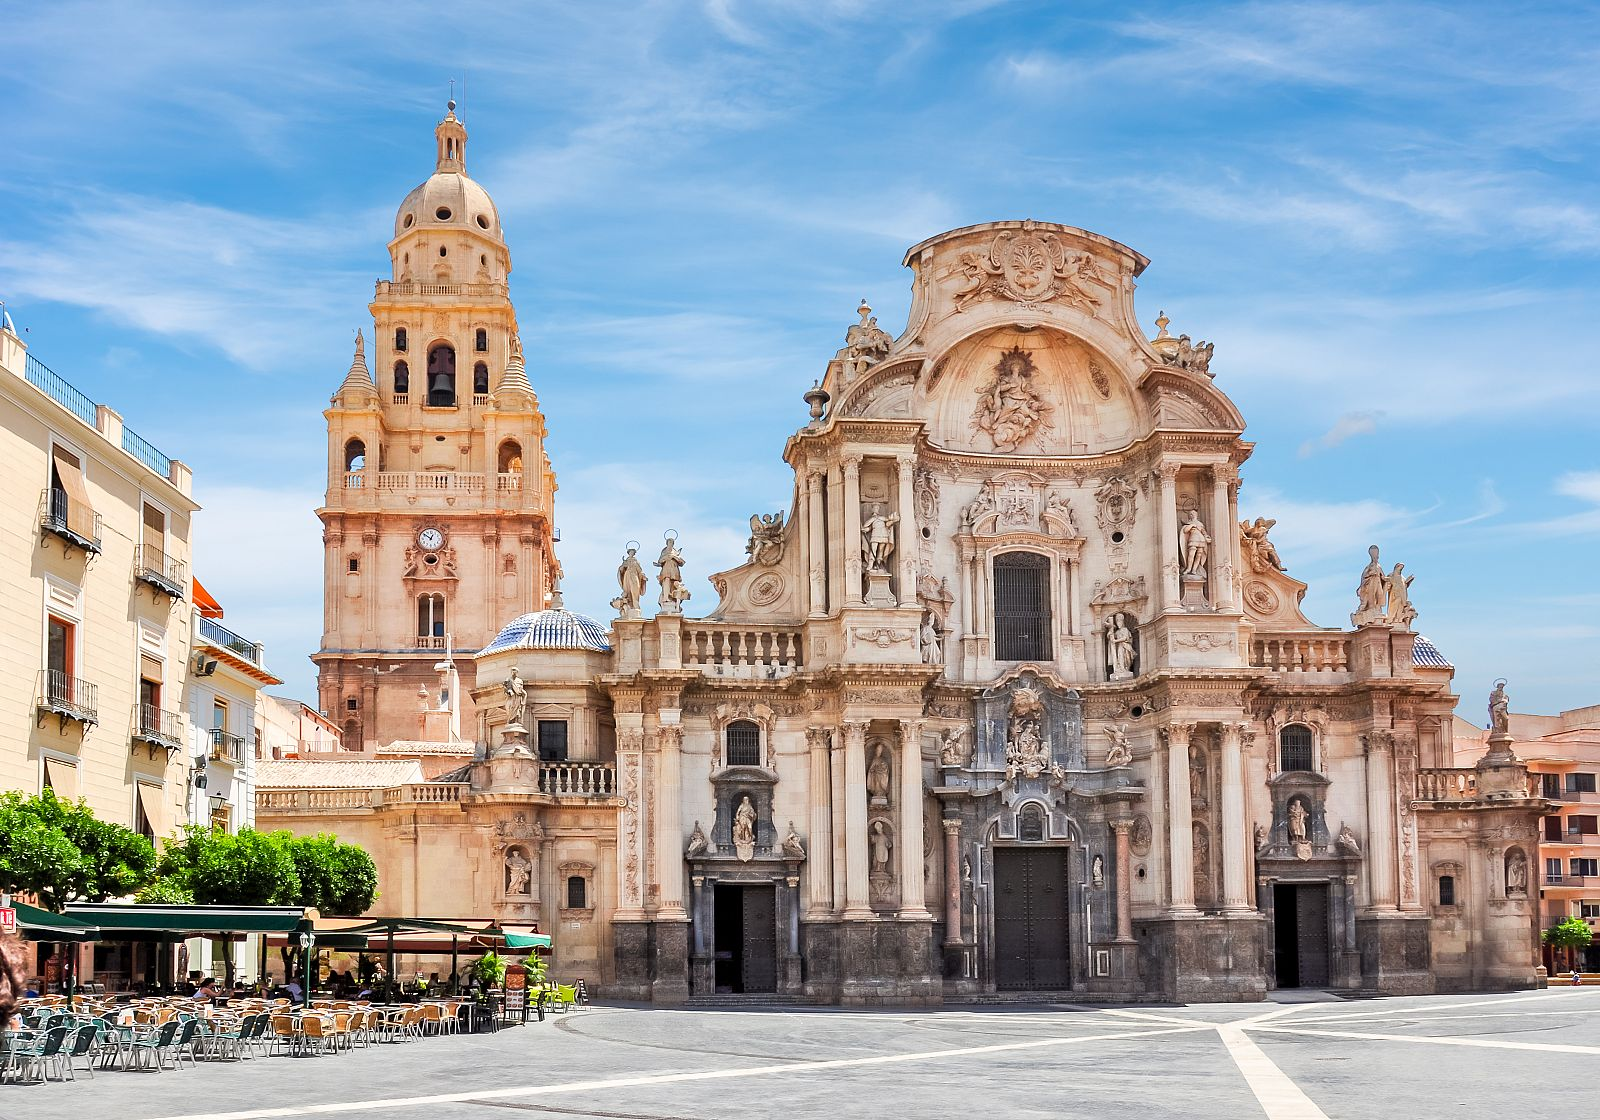
\includegraphics[width=\linewidth]{Figures/catedral.jpg}
    \caption[La catedral más bonita del mundo]{Ilustración de la catedrál más bonita del mundo).}
    \label{fig:figure-01}
\end{figure}

Si deseas comparar imágenes u organizarlas una al lado de la otra, puedes utilizar los entornos \verb|\begin{figure}| y \verb|\begin{subfigure}| de forma conjunta. Luego, puedes referenciar las subfiguras como \autoref{fig:figure-02.1} y \autoref{fig:figure-02.2}.

\begin{figure}[!htpb]
    \centering
    \begin{subfigure}{0.45\textwidth}
        \centering
        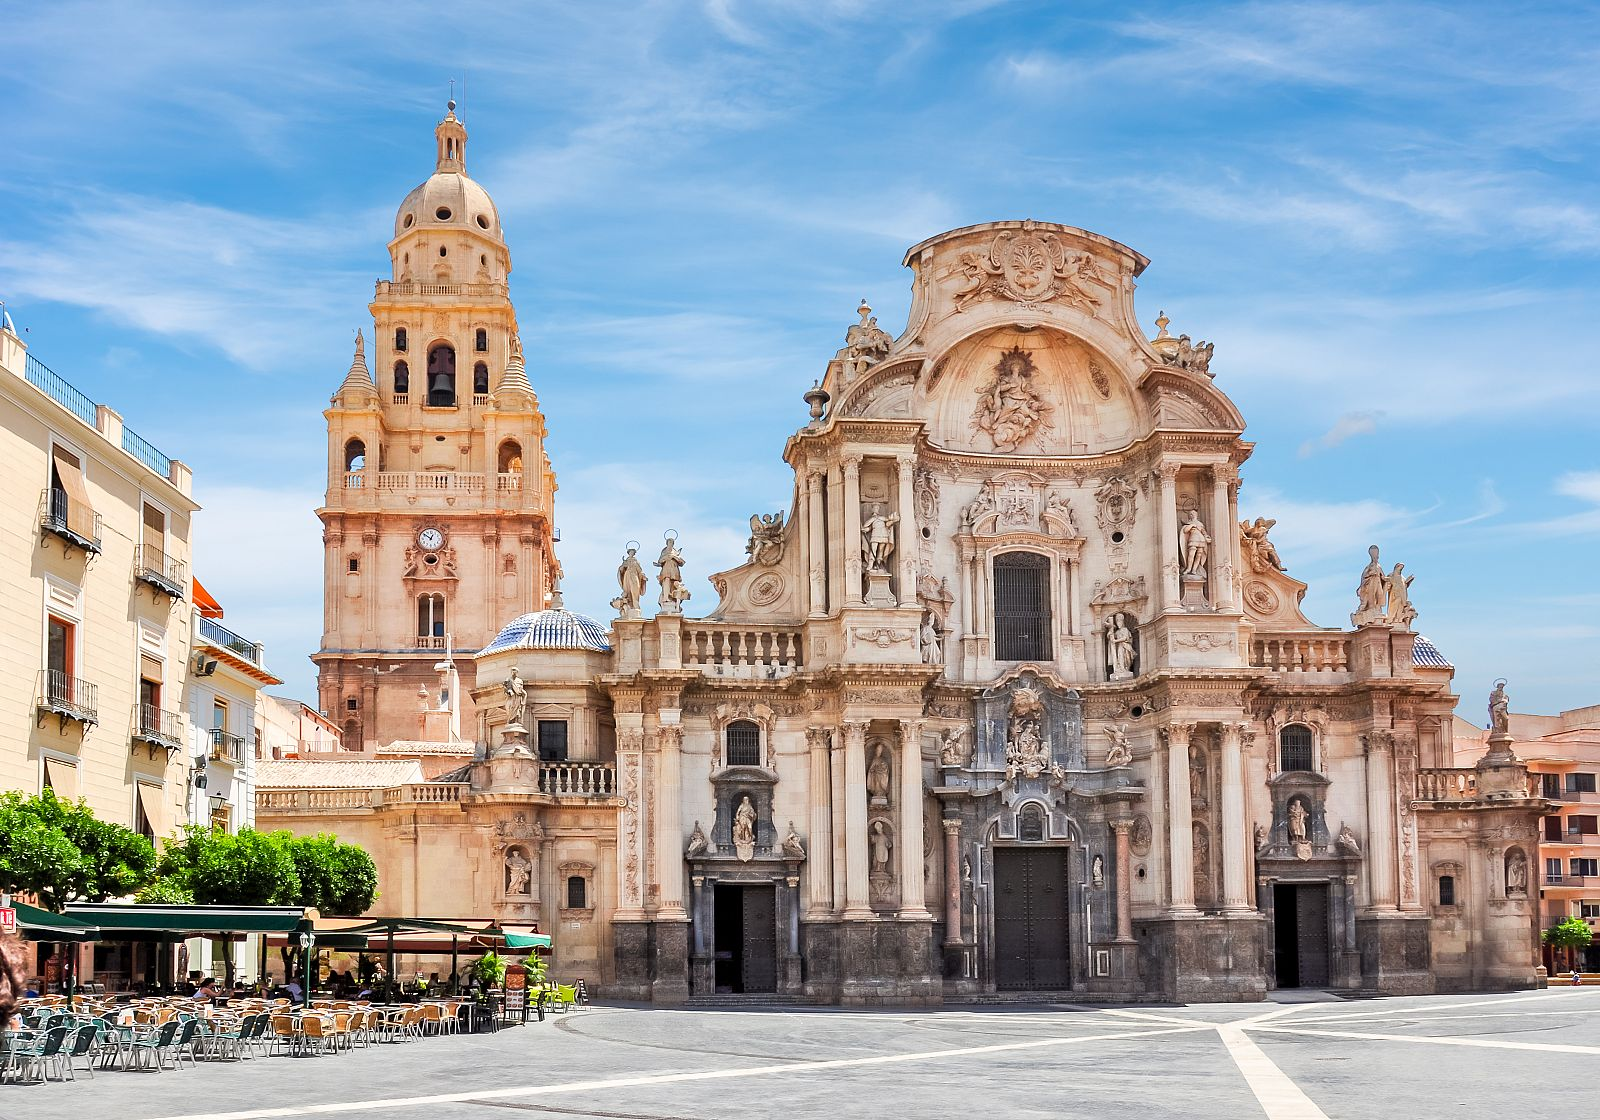
\includegraphics[width=0.9\textwidth]{Figures/catedral.jpg}
        \caption{Subfigura 1.}
        \label{fig:figure-02.1}
    \end{subfigure}
    \hspace{.5cm}
    \begin{subfigure}{0.45\textwidth}
        \centering
        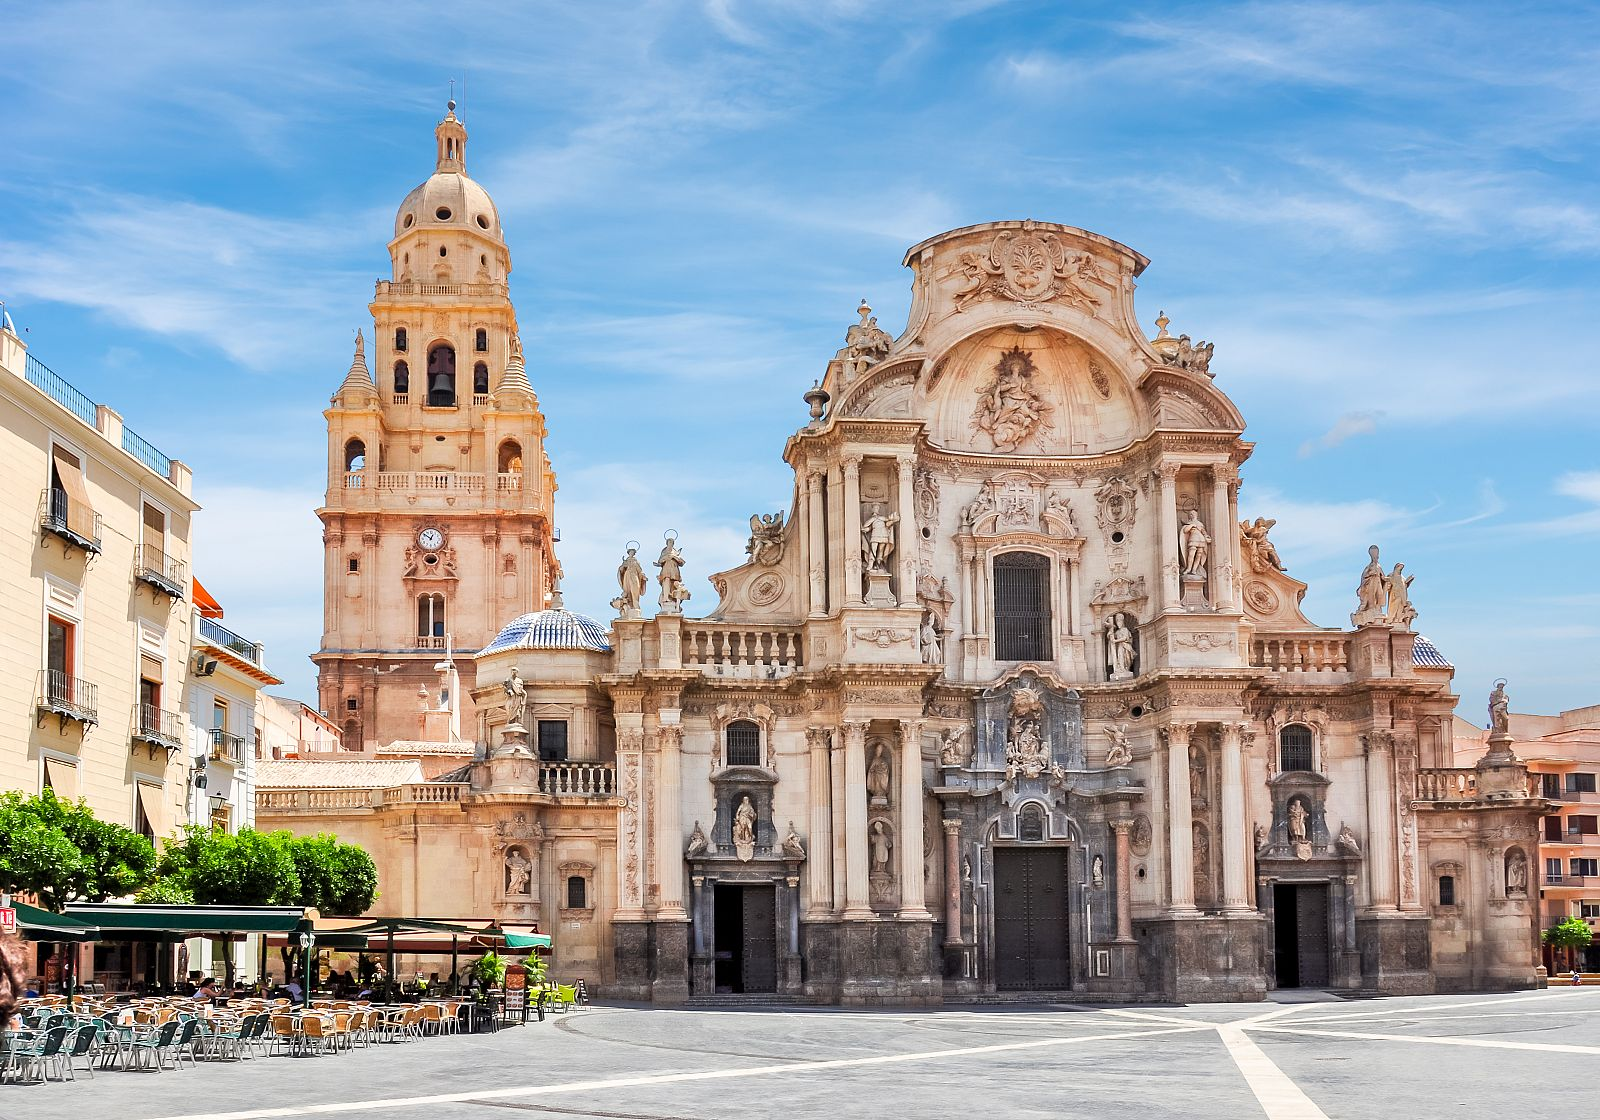
\includegraphics[width=0.9\textwidth]{Figures/catedral.jpg}
        \caption{Subfigura 2.}
        \label{fig:figure-02.2}
    \end{subfigure}
    \caption{La catedral más bonita del mundo.}
    \label{fig:figure-02}
\end{figure}

\section{Tablas}

Las tablas son esenciales para presentar resultados e información de forma clara. En esta sección se presentan distintas técnicas para mostrar datos utilizando los entornos disponibles en esta plantilla. Aunque definir tablas en \LaTeX pueda parecer complicado al principio, esta plantilla simplifica considerablemente el proceso.

\begin{block}[tip]
\textit{Antes de mostrar los diferentes entornos de tablas, es importante recordar que todas deben estar dentro del entorno \texttt{\textbackslash begin\{table\}}. Además, se recomienda utilizar la opción de flotación \texttt{[!htpb]} para mejorar la colocación automática de las tablas en el documento. \textbf{Este consejo también aplica al uso de figuras.}}
\end{block}

\subsection{Entorno Tabular}

El entorno estándar \verb|\begin{tabular}| permite crear tablas simples pero elegantes. La tabla \autoref{tab:table-01} se ha generado utilizando un entorno centrado (\verb|\centering|) y empleando el paquete \verb|booktabs| para mejorar el estilo visual.

\begin{table}[!htpb]
    \caption{Ejemplo de uso del entorno tabular.}
    \label{tab:table-01}
    \centering
    \begin{tabular}{llc}
        \toprule
        \textbf{Encabezado 1} & \textbf{Encabezado 2} & \textbf{Encabezado 3} \\
        \midrule
        Lorem Ipsum         & Pharetra Dolor    & $\checkmark$  \\
        Amet Consectetuer   & Curabitur Aliquet & -             \\
        Praesent Mauris     & Praesent Libero   & $\checkmark$  \\
        \bottomrule
    \end{tabular}
\end{table}


\subsection{Entorno Tabularx}

El paquete \verb|tabularx| permite construir tablas con columnas que se expanden automáticamente para ocupar todo el ancho disponible. Para lograr este comportamiento, se puede utilizar el entorno: \verb|\begin{tabularx}{\textwidth}{lX}|, donde la columna \verb|X| se comporta como una columna multicolumna que ocupa el espacio restante. La tabla \autoref{tab:table-02} muestra un ejemplo del uso de este entorno.

\begin{table}[!htpb]
    \caption{Ejemplo del uso del entorno tabularx.}
    \label{tab:table-02}
    \begin{tabularx}{\textwidth}{lX}
        \toprule
        \textbf{Encabezado 1} & \textbf{Encabezado 2} \\ 
        \midrule
        Foo Bar Baz & Quisque cursus, metus vitae pharetra auctor, sem massa mattis sem, at interdum magna augue eget diam. \\
        Ipsum Dolor & Vestibulum ante ipsum primis in faucibus orci luctus et ultrices posuere cubilia Curae; Curabitur aliquet quam id dui. \\
        Dolor Sit & Phasellus condimentum elementum justo, quis interdum est sagittis ac. Vestibulum non arcu sit amet justo lobortis semper. \\
        Amet Consectetuer & Integer nec odio praesent libero sed cursus ante dapibus diam sed nisi vestibulum non arcu. \\
        Consectetuer Adipiscing & Nulla quis sem at nibh elementum imperdiet. Duis sagittis ipsum. Praesent mauris. \\
        \bottomrule
    \end{tabularx}
\end{table}

\subsection{Entorno Longtable}

Cuando se trabaja con tablas especialmente largas que necesitan dividirse en varias páginas, es conveniente usar el entorno \verb|\begin{longtable}|. Este entorno requiere definir el encabezado dos veces: una para la primera aparición de la tabla y otra para las siguientes páginas. Esto garantiza que el lector pueda identificar correctamente las columnas en todo momento. Consulta la \autoref{tab:table-03} para ver un ejemplo detallado.

\begin{longtable}[c]{lll}
\caption{Ejemplo del uso del entorno longtable.}
\label{tab:table-03} \\
\toprule
\textbf{Nombre} & \textbf{Correo electrónico} & \textbf{Rol o puesto} \\ 
\midrule
\endfirsthead

\multicolumn{3}{c}%
{{\textit{\bfseries Tabla \thetable\ continuación de la página anterior.}}} \\
\toprule
\textbf{Nombre} & \textbf{Correo electrónico} & \textbf{Rol o puesto} \\ 
\midrule
\endhead

\bottomrule
\addlinespace[1mm]
\multicolumn{3}{r}%
{{\textit{Continúa en la siguiente página.}}} \\
\endfoot
\bottomrule
\endlastfoot

Alice Johnson & alice.johnson@email.com & Project Manager \\
Bob Thompson & bob.thompson@email.com & Data Analyst \\
Charlie Davis & charlie.davis@email.com & Marketing Specialist \\
% (continúa con el resto de la tabla...)
Steven Martin & steven.martin@email.com & Robotics Engineer \\
\end{longtable}

\subsection{Tablas Complejas}

Crear tablas complejas en \LaTeX puede ser una tarea algo desafiante. Por ello, se recomienda encarecidamente el uso de herramientas como \href{https://www.tablesgenerator.com/}{Table Generator}. Esta herramienta permite diseñar visualmente la tabla con el estilo deseado y luego copiar fácilmente el código generado al documento LaTeX. 

Este enfoque simplifica el proceso y asegura una representación precisa del contenido. No obstante, es fundamental que la tabla siga siendo comprensible para el lector. \textbf{El exceso de complejidad puede dificultar la interpretación}. La \autoref{tab:table-04} muestra un ejemplo de tabla con múltiples niveles de detalle.

\begin{table}[!htpb]
    \caption{Ejemplo del uso de tablas complejas.}
    \label{tab:table-04}
    \centering
    \begin{tabular}{lcc}
        \toprule
        \multirow{2}{*}{\textbf{Componente}} & \multicolumn{2}{c}{\textbf{Especificaciones}} \\
        \cmidrule(lr){2-3}
        & \textbf{Característica} & \textbf{Compatible} \\
        \midrule
        \multirow{4}{*}{CPU} & Núcleos (ej.: 8) & $\checkmark$ \\
        & Frecuencia base (ej.: 3.6 GHz) & $\checkmark$ \\
        & Hyper-Threading & $\checkmark$ \\
        & Gráficos integrados & - \\
        \midrule
        \multirow{4}{*}{GPU} & Núcleos CUDA (ej.: 5120) & $\checkmark$ \\
        & Frecuencia base (ej.: 1.5 GHz) & $\checkmark$ \\
        & Soporte Ray Tracing & $\checkmark$ \\
        & Multi-GPU (SLI/CrossFire) & - \\
        \midrule
        \multirow{4}{*}{Memoria} & Tipo (ej.: DDR5, GDDR6) & $\checkmark$ \\
        & Capacidad (ej.: 16 GB) & $\checkmark$ \\
        & Ancho de banda (ej.: 448 GB/s) & $\checkmark$ \\
        & Soporte ECC & - \\
        \midrule
        \multirow{3}{*}{Placa Base} & Soporte PCIe 5.0 & $\checkmark$ \\
        & Wi-Fi 6E & $\checkmark$ \\
        & Thunderbolt 4 & - \\
        \bottomrule
    \end{tabular}
\end{table}

\section{Listas}

Crear listas en \LaTeX es sencillo y ofrece varias opciones según tus necesidades. Puedes generar listas con viñetas mediante el entorno \verb|\begin{itemize}| o listas numeradas con \verb|\begin{enumerate}|. A continuación se muestra un ejemplo con el entorno \verb|itemize|:

\begin{itemize}
  \item Cada elemento comienza con el comando \verb|\item|.
  \item Los elementos están marcados con un punto negro (viñeta).
  \item El texto de cada elemento puede tener cualquier longitud.
\end{itemize}

Como se mencionó anteriormente, también puedes crear una lista numerada con el entorno \verb|enumerate|. Por ejemplo:

\begin{enumerate}
  \item Los elementos se numeran automáticamente.
  \item La numeración comienza en 1 en cada entorno \verb|enumerate|.
  \item Otro elemento más en la lista.
\end{enumerate}

También es posible anidar listas dentro de otras listas del mismo tipo. Aquí tienes un ejemplo:

\begin{enumerate}
    \item Elemento de primer nivel
    \item Elemento de primer nivel
    \begin{enumerate}
        \item Elemento de segundo nivel
        \item Elemento de segundo nivel
        \begin{enumerate}
            \item Elemento de tercer nivel
            \item Elemento de tercer nivel
        \end{enumerate}
    \end{enumerate}
\end{enumerate}

\begin{block}[tip]
\textit{Observa que las etiquetas cambian automáticamente según el nivel, aunque se use el mismo entorno para todas las listas. \textbf{Esto demuestra que no es necesario cambiar de entorno para lograr una numeración jerárquica.}}
\end{block}

También puedes personalizar la etiqueta de cada ítem según tus necesidades. Para ello, basta con añadir un nuevo \verb|\item| y colocar la etiqueta deseada entre corchetes. Por ejemplo, \verb|\item[!]| mostrará un signo de exclamación como viñeta. A continuación se muestran algunos ejemplos:

\begin{itemize}
  \item Este es mi primer punto
  \item Otro punto que quiero destacar
  \item[!] ¡Un punto importante!
  \item[$\blacksquare$] Un punto fuerte y cuadrado
  \item[] ¿Una etiqueta vacía?
\end{itemize}

Por último, puedes utilizar una lista descriptiva. A diferencia de las listas con viñetas o numeradas, este tipo permite asignar una descripción personalizada a cada elemento. En el siguiente ejemplo, hay tres entradas: dos con descripción y una sin etiqueta:

\begin{description}
    \item[Elemento 1:] Este es el primer ítem con descripción.
    \item[Elemento 2:] Otro ítem con una descripción diferente.
    \item Un ítem sin una etiqueta específica.
\end{description}

\section{Listados de Código}

A veces puede ser útil incluir fragmentos de código fuente directamente en tu documento. Para ello, puedes usar dos entornos anidados: \verb|\begin{listing}|, que permite añadir título y etiqueta, y \verb|\begin{minted}|, que aplica resaltado de sintaxis.

\autoref{listing:c-code} muestra un ejemplo de código en lenguaje C:

\begin{listing}[!htpb]
\caption{Hola mundo en C.}
\label{listing:c-code}
\begin{minted}{c}
#include <stdio.h>
int main() {
   printf("Hello, World!"); /* printf() imprime la cadena */
   return 0;
}
\end{minted}
\end{listing}

El código anterior está incluido directamente en el documento. Sin embargo, también puedes importar código desde un archivo externo. Para ello, utiliza el comando \verb|\inputminted{LENGUAJE}{ARCHIVO}| dentro del entorno \verb|listing|. En el siguiente ejemplo, se importa código Haskell:

\begin{listing}[!htpb]
\caption{Factorial en Haskell.}
\label{listing:haskell-code}
\inputminted{haskell}{Code/Factorial.hs}
\end{listing}

En algunos casos, cuando solo necesitas resaltar un comando específico, no es necesario usar \verb|listing| ni \verb|minted|. Puedes usar el comando \verb|\verb| para resaltar texto en línea o \verb|\begin{verbatim}| para bloques largos.

Ejemplo:

\begin{verbatim}
\begin{listing}[!htpb]
    \inputminted{LENGUAJE}{ARCHIVO}
    \caption{TÍTULO}
    \label{ETIQUETA}
\end{listing}
\end{verbatim}

Si el fragmento de código es demasiado largo y ocupa varias páginas, puedes usar el entorno \verb|\begin{longlisting}|, que divide automáticamente el contenido en varias páginas. Un ejemplo se muestra en \autoref{listing:lisp-code}.

\begin{longlisting}
\caption{Ejemplo de funciones en Lisp.}
\label{listing:lisp-code}
\begin{minted}{lisp}
(defun factorial (n)
  "Calcula el factorial de un número."
  (if (zerop n)
      (* n (factorial (1- n)))))

(defun fibonacci (n)
  "Calcula el n-ésimo número de Fibonacci."
  (cond ((zerop n) 0)
        ((= n 1) 1)
        (t (+ (fibonacci (1- n)) (fibonacci (- n 2))))))

(defun gcd (a b)
  "Calcula el máximo común divisor entre a y b."
  (if (zerop b)
      a
      (gcd b (mod a b))))

(defun primes-up-to (limit)
  "Devuelve una lista de todos los números primos hasta LIMIT."
  (let ((primes '()))
    (loop for i from 2 to limit
          unless (some (lambda (p) (zerop (mod i p))) primes)
          do (push i primes))
    (nreverse primes)))

(defun example-function (x)
  "Función de ejemplo para demostrar capacidades en Lisp."
  (let ((result (list (factorial x)
                      (fibonacci x)
                      (gcd x 10)
                      (primes-up-to x))))
    (format t "Factorial de ~A: ~A~%" x (factorial x))
    (format t "Fibonacci de ~A: ~A~%" x (fibonacci x))
    (format t "MCD de ~A y 10: ~A~%" x (gcd x 10))
    (format t "Primos hasta ~A: ~A~%" x (primes-up-to x))
    result))

(example-function 10)
\end{minted}
\end{longlisting}

\section{Ecuaciones}

Al redactar ecuaciones o expresiones matemáticas, \LaTeX es una herramienta potente y versátil. Puedes introducir fórmulas en modo en línea usando el entorno \verb|\(FORMULA\)| o utilizar \verb|\begin{equation}| para mostrar la ecuación en modo matemático con numeración. Si prefieres que la ecuación no tenga numeración, puedes usar el entorno \verb|\[FORMULA\]|.

\vspace{.875em}
\textbf{Ejemplo:} En física, la equivalencia entre masa y energía se expresa mediante la ecuación \(E=mc^2\), descubierta en 1905 por Albert Einstein. En unidades naturales ($c = 1$), la fórmula (\ref{eq:equation-01}) expresa la siguiente identidad:

\begin{equation}
\label{eq:equation-01}
E = m.c^2
\end{equation}

\textbf{Ejemplo:} A continuación se muestra una ecuación —\textit{sin numeración}— que representa una función de pérdida regularizada en aprendizaje supervisado, combinando la pérdida media de predicción sobre el conjunto de entrenamiento y un término de regularización $L_2$ para evitar el sobreajuste:

\[
\mathcal{L}(\boldsymbol{\theta}) = \frac{1}{N} \sum_{i=1}^{N} \ell(y_i, f(\mathbf{x}_i; \boldsymbol{\theta})) + \lambda \|\boldsymbol{\theta}\|_2^2
\]

Crear ecuaciones puede resultar complejo, por lo que recomendamos usar un editor en línea como \href{https://latexeditor.lagrida.com/}{LaTeX Equation Editor}. Solo tienes que construir la fórmula, copiarla y pegarla en tu documento, ya sea en línea o en un bloque matemático.

\section{Notas al pie}

En ocasiones, puede ser útil presentar información complementaria que no forma parte del cuerpo principal del texto. En \LaTeX, esto se puede hacer fácilmente usando el comando \verb|\footnote{TEXTO}|. El contenido aparecerá al pie de la página\footnote{Esto es una nota.}.

Si deseas insertar notas al pie dentro de una tabla, es mejor replantearlo, ya que \LaTeX no ofrece una forma sencilla de manejarlas. En su lugar, puedes colocar un asterisco “*” donde quieras que aparezca la referencia. Luego, debajo de la tabla —\textbf{pero antes de cerrar el entorno \texttt{table}}— coloca el texto asociado al asterisco. Así lograrás un efecto similar al de una nota al pie, pero localizada bajo la tabla y no al final de la página.


%%% Discusión %%%

\include{Chapters/07-Discussion}

%%% Conclusiones %%%

\include{Chapters/08-Conclusions}

%%% Bibliography %%%
\renewcommand{\refname}{Bibliography}
\printbibliography[title={\refname},heading=bibintoc]

%%% Appendices: Work that *YOU* Developed %%%
\appendix
\ifthenelse{\equal{\LanguageOption}{spanish}}{
    \addtocontents{toc}{\protect\contentsline{chapter}{Apéndices}{}{}}
}{
    \addtocontents{toc}{\protect\contentsline{chapter}{Appendices}{}{}}
}

\ifthenelse{\equal{\MediaOption}{paper}}{\blankpage}{\clearpage}
\begin{center}
    \crimsonfont
    \thispagestyle{empty}
        
    \vspace*{\fill}
    \ifthenelse{\equal{\LanguageOption}{spanish}}{%
        {\LARGE\fontsize{26}{26}\selectfont\textcolor{maincolor}{Apéndices}\par}
    }{%
        {\LARGE\fontsize{26}{26}\selectfont\textcolor{maincolor}{Appendices}\par}
    }
    \vspace*{\fill}
\end{center}
\MediaOptionLogicBlank
\chapter{Showcasing the First Appendix}
\guideinfo{Appendices contain supplementary material \textbf{created by the author} that enhances the reader’s understanding of the dissertation while not being essential for following the primary narrative. These sections often include detailed tables, figures, complex calculations, or materials like survey questions and interview transcripts produced in the course of the research. The appendices allow readers to explore the research in greater detail, offering a deeper insight into methods and findings without interrupting the main body of work.}
%% Recommended dimensions for a landscape layout; adjust as needed.
\begin{landscapemode}{297mm}{420mm}
    \chapter{Showcasing the Second Appendix}
    \blindtext[5]
\end{landscapemode}

%%% Annexes: Work that *YOU DID NOT* Develop %%%
\ifthenelse{\equal{\LanguageOption}{spanish}}{
    \addtocontents{toc}{\protect\contentsline{chapter}{Anexos}{}{}}
}{
    \addtocontents{toc}{\protect\contentsline{chapter}{Annexes}{}{}}
}

\setcounter{chapter}{11} % To start at the "L" chapter.
\MediaOptionLogicAnnexes
\begin{center}
    \crimsonfont
    \thispagestyle{empty}
        
    \vspace*{\fill}
    \ifthenelse{\equal{\LanguageOption}{spanish}}{%
        {\LARGE\fontsize{26}{26}\selectfont\textcolor{maincolor}{Anexos}\par}
    }{%
        {\LARGE\fontsize{26}{26}\selectfont\textcolor{maincolor}{Annexes}\par}
    }
    \vspace*{\fill}
\end{center}
\MediaOptionLogicBlank
\chapter{Showcasing the First Annex}
\guideinfo{Annexes are supplementary sections in a dissertation that provide additional information or external documents not essential to the main arguments but that support or complement the research. Unlike appendices, \textbf{annexes generally contain material that was not developed by the author}, such as reports, legal documents, or published datasets from external sources. This information is placed separately to keep the main content concise, allowing readers access to relevant external references without disrupting the dissertation's flow.}

%%% Back Page %%%
\ifthenelse{\equal{\MediaOption}{paper}}{\blankpage}{}

\clearpage
\null
\thispagestyle{empty}

% Back page

       \newcommand\BackgroundPicBackPage{%
    \put(0,0){%
    \parbox[b][\paperheight]{\paperwidth}{%
    \vfill
    \centering
    
\includegraphics[width=\paperwidth,height=\paperheight,keepaspectratio]{Figures/Theme/Back-Page-BG.pdf}%
    \vfill
    }}}


\AddToShipoutPictureBG*{\BackgroundPicBackPage}

\newgeometry{margin=1.98cm, top=1.47cm, bottom=1.47cm}
\noindent\clearpage
\restoregeometry

\end{document}